% The document class
\documentclass[a4paper, 12pt]{report}

% The geometry of the pages
\usepackage[a4paper, margin=25mm]{geometry}

% For maths
\usepackage{amsmath}
\usepackage{amsfonts}
\usepackage{amssymb}
\usepackage{mathpartir}

% For algorithms
\usepackage{algpseudocode}

% For lists
\usepackage{enumitem}
\usepackage{listings}

% For trees
\usepackage{qtree}

% For hyperlinks
\usepackage{hyperref}

% For formatting columns in a table
\usepackage{array}

\newcolumntype{L}[1]{>{\raggedright\let\newline\\\arraybackslash\hspace{0pt}}m{#1}}
\newcolumntype{C}[1]{>{\centering\let\newline\\\arraybackslash\hspace{0pt}}m{#1}}
\newcolumntype{R}[1]{>{\raggedleft\let\newline\\\arraybackslash\hspace{0pt}}m{#1}}

% For centering wide tables.
\usepackage{adjustbox}

% For graphics and colour
\usepackage{graphicx}
\usepackage{color}

% For plotting graphs.
\usepackage{pgfplots}

% For centering captions.
\usepackage{caption}

% For temporarily splitting the document into multiple columns
\usepackage{multicol}

% For circuit/logic diagrams
\usepackage{circuitikz}

% Enables spacing in file paths when inserting images
\usepackage[space]{grffile}

% Remove paragraph indentation
\setlength\parindent{0pt}

% The colours used by lstlisting
\definecolor{mygreen}{rgb}{0,0.6,0}
\definecolor{mygray}{rgb}{0.5,0.5,0.5}
\definecolor{mymauve}{rgb}{0.58,0,0.82}

% For blocks of code
\lstset{ %
  aboveskip=1em,
  backgroundcolor=\color{white},	% choose the background color; you must add \usepackage{color} or \usepackage{xcolor}
  basicstyle=\ttfamily\scriptsize,		% the size of the fonts that are used for the code
  belowskip=-2em,
  breakatwhitespace=false,		% sets if automatic breaks should only happen at whitespace
  breaklines=true,				% sets automatic line breaking
  captionpos=b,					% sets the caption-position to bottom
  commentstyle=\color{mygreen},	% comment style
  deletekeywords={...},			% if you want to delete keywords from the given language
  escapeinside={\%*}{*)},			% if you want to add LaTeX within your code
  extendedchars=true,			% lets you use non-ASCII characters; for 8-bits encodings only, does not work with UTF-8
  frame=single,					% adds a frame around the code
  keepspaces=true,				% keeps spaces in text, useful for keeping indentation of code (possibly needs columns=flexible)
  keywordstyle=\color{blue},		% keyword style
  language=Java,				% the language of the code
  otherkeywords={},				% if you want to add more keywords to the set, e.g. for ML you might have {fun, let, ...}
  numbers=left,					% where to put the line-numbers; possible values are (none, left, right)
  numbersep=5pt,				% how far the line-numbers are from the code
  numberstyle=\tiny\color{mygray},	% the style that is used for the line-numbers
  rulecolor=\color{black},			% if not set, the frame-color may be changed on line-breaks within not-black text (e.g. comments (green here))
  showspaces=false,				% show spaces everywhere adding particular underscores; it overrides 'showstringspaces'
  showstringspaces=false,			% underline spaces within strings only
  showtabs=false,				% show tabs within strings adding particular underscores
  stepnumber=1,				% the step between two line-numbers. If it's 1, each line will be numbered
  stringstyle=\color{mymauve},		% string literal style
  tabsize=2,					% sets default tabsize to 2 spaces
  title=\lstname					% show the filename of files included with \lstinputlisting; also try caption instead of title
}

% Defines \ip{arg1}{arg2} to mean (arg1, arg2).
\newcommand{\ip}[2]{(#1, #2)}

% Horizontal rule command used for title
\newcommand{\horrule}[1]{\rule{\linewidth}{#1}}

% TO DO macro
\newcommand{\todo}{\textbf{\textit{\textcolor{red}{TODO: }}}}

% Shorten textbf
\newcommand{\tbf}[1]{\textbf{#1}}

% Shorten texttt
\newcommand{\ttt}[1]{\texttt{#1}}

% Shorten textit
\newcommand{\tit}[1]{\textit{#1}}

% Blue, underlined hyperlinks
\newcommand{\hlink}[2]{{\href{#1}{#2}}}

% Bullet point
\newcommand{\bpt}[0]{\textbullet~}

% White bullet point
\newcommand{\wbpt}[0]{$\circ$~}

% \cmark and \xmark can be used as a tick and a cross respectively
\newcommand{\cmark}{\ding{51}}
\newcommand{\xmark}{\ding{55}}

% Set the Table of Contents depth.
\setcounter{tocdepth}{2}

\begin{document}

\begin{titlepage}
	\noindent
	\begin{minipage}[t][][t]{0.5\textwidth}
		
\includegraphics[width=40mm]{./Images/CamLogo.jpg}
	\end{minipage}
	\begin{minipage}{0.5\textwidth}
	\begin{flushright}
		\large
		\textit{Devan Kuleindiren}
		\\
		\textit{Robinson College}
		\\
		\texttt{dk503}
	\end{flushright}
	\end{minipage}
	
	\begin{center}
	\vspace{6cm}
	{\scshape\large Computer Science Tripos - Part II Project\par}
	\vspace{0.5cm}
	{\huge\bfseries Language Modelling for Text Prediction\par}
	\vspace{0.5cm}
	{\large \today \par}
	\end{center}
	
	\vfill
	
	\begin{center}
	supervised by \\
	Dr Marek Rei \& Dr Ekaterina Shutova
	\end{center}
	
	\vspace{1.5cm}
\end{titlepage}

% Proforma, table of contents and list of figures

\pagestyle{plain}

\chapter*{Proforma}

{\large
\begin{tabular}{ll}
Name:               & \bf Devan Kuleindiren \\
College:            & \bf Robinson College \\
Project Title:      & \bf Language Modelling for Text Prediction \\
Examination:        & \bf Computer Science Tripos -- Part II, June 2017 \\
Word Count:         & \bf ? \\
Project Originator: & Devan Kuleindiren \& Dr Marek Rei \\
Supervisors:         & Dr Marek Rei \& Dr Ekaterina Shutova \\
\end{tabular}
}
\stepcounter{footnote}

\section*{Original Aims of the Project}
The primary aim of the project was to implement and benchmark a variety of language models, comparing the quality of their predictions as well as the time and space that they consume. More specifically, I aimed to build an $n$-gram language model along with several smoothing techniques, and a variety of recurrent neural network-based language models. An additional aim was to investigate ways to improve the performance of existing language models on error-prone text.

\section*{Work Completed}
All of the project aims set out in the proposal have been met, resulting in a series of language model implementations and a generic benchmarking framework for comparing their performance. I have also proposed and evaluated a novel extension to an existing language model which improves its performance on error-prone text. Additionally, as an extension, I implemented a mobile keyboard on iOS that uses my language model implementations as a library.

\section*{Special Difficulties}
None.

 
\newpage
\section*{Declaration}

I, Devan Kuleindiren of Robinson College, being a candidate for Part II of the Computer Science Tripos, hereby declare that this dissertation and the work described in it are my own work, unaided except as may be specified below, and that the dissertation does not contain material that has already been used to any substantial extent for a comparable purpose.

\vspace{1cm}
\begin{multicols}{2}

\rule{5cm}{0.15mm} \\
\leftline{\scshape{Signed}}

\columnbreak

\rule{5cm}{0.15mm} \\
\leftline{\scshape{Date}}

\end{multicols}


\tableofcontents

\listoffigures


%%%%%%%%%%%%%%%%%%%%%%%%%%%%%%%%%%%%%%%%%%%%%%%%%%%%%%%%%%%%%%%%%%%%%%%
% now for the chapters

\pagestyle{headings}

\chapter{Introduction}

My project investigates the performance of various language models in the context of text prediction. I started by implementing a series of well-established models and comparing their performance, before assessing the tradeoffs that occur when you attempt to apply them in a practical context, such as in a mobile keyboard. Finally, I propose a novel extension to an existing model which aims to improve its performance on error-prone text.

\section{Language Models}

Language models (LMs) produce a probability distribution over a sequence of words, which can be used to estimate the relative likelihood of words or phrases occurring in various contexts. This predictive power is useful in a variety of applications. For example, in speech recognition, if the speech recogniser has estimated two candidate word sequences from an acoustic signal \tit{`it's not easy to wreck a nice beach'} and \tit{`it's not easy to recognise speech'}, then a language model can be used to determine that the second candidate is more probable than the first. Language models are also used in machine translation, handwriting recognition, part-of-speech tagging and information retrieval.

\begin{alignat*}{2}
	\overbrace{\tit{Do you want to grab a }}^{w_1^k}&\overbrace{\underline{\tit{drink}}}^{w_{k+1}} &&\hspace{0.5mm}\overbrace{(0.327)}^{\mathbb{P}(w_{k + 1} | w_1^k)} \\
	&\tit{coffee} &&\ \ (0.211) \\
	&\tit{bite} &&\ \ (0.190) \\
	&\tit{spot} &&\ \ (0.084) \\
	&\vdots &&\ \ \vdots
\end{alignat*}

My project focuses on language modelling in the context of text prediction. That is, given a sequence of words $w_1w_2...w_k = w_1^k$, I want to estimate $\mathbb{P}(w_{k + 1} | w_1^k)$. For instance, if a user has typed \tit{`do you want to grab a '}, then a language model could be used to suggest probable next words such as \tit{`coffee'}, \tit{`drink'} or \tit{`bite'}, and these predictions could further be narrowed down as the user continues typing.

\section{Motivation}


\subsection*{Benchmarking}

\begin{itemize}
\item
	Variety of language models, that vary in accuracy, memory consumption and speed.
\item
	Combinations can be considered.
\item
	Important tradeoffs when applying them to mobile.
\end{itemize}

There are two prominent approaches to language modelling, the first of which is the $n$-gram approach and the second of which is based on (recurrent) neural networks.

 language models and their various smoothing techniques, before proceeding onto neural network-based language models. Combinations of such models, which can be achieved by interpolating their probability distributions, will also be included in the benchmark. \\

New techniques for facilitating better predictions are constantly being developed for language models. However, it is important to realise that such models are being used increasingly in a mobile environment, where the computational and memory resources aren't as abundant.

\subsection*{Error-prone Text}

One problem with existing language models is that their next-word predictions tend to be less accurate when they are presented with error-prone text. This isn't surprising, because they are only ever trained on sentences that do not contain any errors.

Unfortunately, humans are not perfect, and they will make typographical mistakes, spelling mistakes and occasionally grammatical errors too. In this project I investigate ways to bridge the gap in performance between language model predictions on error-prone text and error-free text. 

\section{Related Work}
\begin{itemize}
\item
	Google 1-Billion Word benchmark
\item
	Chen and Goodman smoothing paper
\item
	Work that's been done on language models with error-prone text 
\end{itemize}

\chapter{Preparation}

My preparation consisted of thoroughly understanding $n$-gram and RNN-based language models, as well as planning how to tie them all together in an efficient implementation.

\section{$n$-gram Models}

This section describes $n$-gram language models and the various smoothing techniques implemented in this project.

\subsection{An Overview of $n$-gram Models}

Language models are concerned with the task of computing $\mathbb{P}(w_1^N)$, the probability of a sequence of words $w_1w_2...w_N = w_1^N$, where $w_i \in V$ and $V$ is some predefined vocabulary\footnote{The vocabulary is typically taken as all of the words that occur at least $k$ times in the training set. $k$ is typically around 2 or 3.}. By repeated application of the product rule, it follows that:
\begin{gather*}
	\mathbb{P}(w_1^N) = \prod_{i = 1}^N \mathbb{P}(w_i | w_1^{i - 1})
\end{gather*}
$n$-gram language models make the Markov assumption that $w_i$ only depends on the previous $(n - 1)$ words. That is, $\mathbb{P}(w_i | w_1^{i - 1}) \approx \mathbb{P}(w_i | w_{i - n + 1}^{i - 1})$:
\begin{gather*}
	\mathbb{P}(w_1^N) \approx \prod_{i = 1}^N \mathbb{P}(w_i | w_{i - n + 1}^{i - 1})
\end{gather*}
Using the maximum likelihood estimation, $\mathbb{P}(w_i | w_{i - n + 1}^{i - 1})$ can be estimated as follows:
\begin{gather*}
	\mathbb{P}(w_i | w_{i - n + 1}^{i - 1})_{MLE} = \frac{c(w_{i - n + 1}^{i})}{\sum_w c(w_{i - n + 1}^{i - 1}w)}
\end{gather*}
where $c(W)$ denotes the number of times that the word sequence $W$ was seen in the training set. \\

To a first approximation, the aforementioned $n$-gram language model provides reasonable results and is simple to compute. However, it does have one major issue: if, as an example, a 3-gram (trigram) model does not encounter the trigram \tit{`the cat sat'} in the data it is trained upon, then it will assign a probability of 0 to that word sequence. This is problematic, because \tit{`the cat sat'} and many other plausible sequences of words might not occur in the training data. In fact, there are $|V|^n$ possible $n$-grams for a language model with vocabulary $V$, which is exponential in the value of $n$. This means that as the value of $n$ is increased, the chances of encountering a given $n$-gram in the training data becomes exponentially less likely. \\

One way to get around this problem is to exponentially increase the size of the training set. This does, however, require significantly more memory and computation, and assumes that additional training data is available in the first place. An alternative solution is to adopt a technique called \tit{smoothing}. The idea behind smoothing is to `smooth' the probability distribution over the words in the vocabulary such that rare or unseen $n$-grams are given a non-zero probability. There are a variety of methods that achieve this. The ones which I have implemented are described in the next section. \\

\begin{figure}[h]
\centering
\captionsetup{justification=centering}
$\vcenter{\hbox{
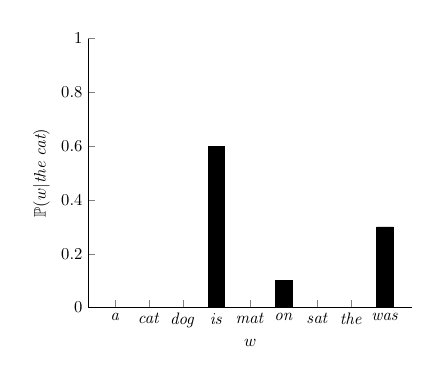
\begin{tikzpicture}[scale=0.6]
\begin{axis}[
	symbolic x coords={\tit{a}, \tit{cat}, \tit{dog}, \tit{is}, \tit{mat}, \tit{on}, \tit{sat}, \tit{the}, \tit{was}},
	xtick=data,
	xlabel={$w$},
	ylabel={$\mathbb{P}(w | \tit{the cat})$},
	ymin=0, ymax=1,
	axis x line*=bottom,
	axis y line*=left,
]

\addplot[ybar, fill=black]
coordinates {(\tit{a}, 0)(\tit{cat}, 0)(\tit{dog}, 0)(\tit{is}, 0.6)(\tit{mat}, 0)(\tit{on}, 0.1)(\tit{sat}, 0)(\tit{the}, 0)(\tit{was}, 0.3)};

\end{axis}
\end{tikzpicture}}}
~~\vcenter{\hbox{\scalebox{1}{$\rightarrow$}}}~~
\vcenter{\hbox{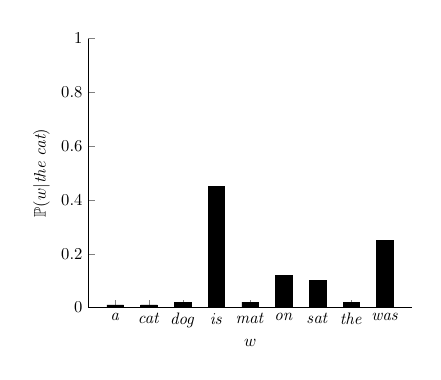
\begin{tikzpicture}[scale=0.6]
\begin{axis}[
	symbolic x coords={\tit{a}, \tit{cat}, \tit{dog}, \tit{is}, \tit{mat}, \tit{on}, \tit{sat}, \tit{the}, \tit{was}},
	xtick=data,
	xlabel={$w$},
	ylabel={$\mathbb{P}(w | \tit{the cat})$},
	ymin=0, ymax=1,
	axis x line*=bottom,
	axis y line*=left,
]

\addplot[ybar, fill=black]
coordinates {(\tit{a}, 0.01)(\tit{cat}, 0.01)(\tit{dog}, 0.02)(\tit{is}, 0.45)(\tit{mat}, 0.02)(\tit{on}, 0.12)(\tit{sat}, 0.1)(\tit{the}, 0.02)(\tit{was}, 0.25)};

\end{axis}
\end{tikzpicture}}}$
\caption{A toy example of smoothing. The probabilities of words that frequently follow \tit{`the cat'} are distributed to other less frequently occurring words in the vocabulary. The vocabulary is $V = \{$\tit{a}, \tit{cat}, \tit{dog}, \tit{is}, \tit{mat}, \tit{on}, \tit{sat}, \tit{the}, \tit{was}$\}$.}
\end{figure}

\subsection{Smoothing Techniques}

\subsubsection{Add-One Smoothing}

Add-one smoothing \cite{add1_smoothing:johnson1932} simply involves adding 1 to each of the $n$-gram counts, and dividing by $|V|$ to ensure the probabilities sum to 1:
\begin{gather*}
	\mathbb{P}(w_i | w_{i - n + 1}^{i - 1})_{\text{\scshape add-one}} = \frac{c(w_{i - n + 1}^{i}) + 1}{\sum_w c(w_{i - n + 1}^{i - 1}w) + |V|}
\end{gather*}
One issue with add-one smoothing is that it gives an equal amount of probability to all $n$-grams, regardless of how likely they actually are. As an example, if both \tit{`the cat'} and \tit{`pizza cat'} are unseen in the training data of a bigram model, then $\mathbb{P}(\tit{cat}\ |\ \tit{the})_{\text{\scshape add-one}} = \mathbb{P}(\tit{cat}\ |\ \tit{pizza})_{\text{\scshape add-one}}$, despite the fact that \tit{`the'} is much more likely to precede \tit{`cat'} than \tit{`pizza'}. This problem can be reduced by employing \tit{backoff}, a technique whereby you recurse on the probability calculated by the $(n - 1)$-gram model. In this case, it is likely that $\mathbb{P}(\tit{the})_{\text{\scshape add-one}} > \mathbb{P}(\tit{pizza})_{\text{\scshape add-one}}$, which could be used to deduce that \tit{`the cat'} is more likely than \tit{`pizza cat'}.

\subsubsection{Absolute Discounting}

Absolute discounting employs backoff by interpolating higher and lower order $n$-gram models. It does this by subtracting a fixed discount $0 \leq D \leq 1$ from each non-zero count:
\begin{equation*}
\begin{aligned}
	\mathbb{P}(w_i | w_{i - n + 1}^{i - 1})_{\text{\scshape ABS}} &= \frac{max\{c(w_{i - n + 1}^{i}) - D, 0\}}{\sum_w c(w_{i - n + 1}^{i - 1}w)} \\
	&+ \frac{D}{\sum_w c(w_{i - n + 1}^{i - 1}w)}N_{1+}(w_{i - n + 1}^{i - 1}\bullet)\mathbb{P}(w_i | w_{i - n + 2}^{i - 1})_{\text{\scshape ABS}}
\end{aligned}
\end{equation*}
where
\begin{gather*}
	N_{1+}(w_{i - n + 1}^{i - 1}\bullet) = |\{ w\ |\ c(w_{i - n + 1}^{i - 1}w) \geq 1 \}|
\end{gather*}
and the base case of recursion $\mathbb{P}(w)_{\text{\scshape ABS}}$ is given by the maximum likelihood unigram model. $N_{1+}(w_{i - n + 1}^{i - 1}\bullet)$ is the number of unique words that follow the sequence $w_{i - n + 1}^{i - 1}$, which is the number of $n$-grams that $D$ is subtracted from. It is not difficult to show that the coefficient attached to the $\mathbb{P}(w_i | w_{i - n + 2}^{i - 1})_{\text{\scshape ABS}}$ term ensures that the probabilities sum to 1. \\

Ney, Essen and Kneser \cite{absolute_discounting:ney1994} suggested setting $D$ to the value:
\begin{gather}
	D = \frac{n_1}{n_1 + 2n_2}
\end{gather}
where $n_1$ and $n_2$ are the total number of $n$-grams with 1 and 2 counts respectively.

\subsubsection{Kneser-Ney Smoothing}

Kneser and Ney proposed an extension to absolute discounting which takes into account the number of unique words that precede a given $n$-gram \cite{kneser_ney_smoothing:kneser1995}. As a motivating example, consider the bigram \tit{`bottle cap'}. If \tit{`bottle cap'} has never been seen in the training data, then the absolute discounting model would backoff onto the unigram distribution for \tit{`cap'}. Using the unigram distribution, \tit{`Francisco'} might be given a higher probability than \tit{`cap'} (assuming \tit{`Francisco'} occurs more frequently than \tit{`cap'}). This would result in the bigram \tit{`bottle Francisco'} being given a higher probability than \tit{`bottle cap'}. Clearly, this is undesirable, because \tit{`Francisco'} only ever follows \tit{`San'}. \\

From this example, it seems intuitive to assign more probability to those $n$-grams that follow a larger number of unique words. Kneser and Ney encapsulate this intuition by replacing some of the absolute counts $c(w_i^j)$ with the number of unique words that precede the word sequence $w_i^j$, $N_{1+}(\bullet w_i^j)$:
\begin{gather*}
	N_{1+}(\bullet w_i^j) = |\{w\ |\ c(w_i^jw) \geq 1\}|
\end{gather*}
Kneser-Ney smoothing\footnote{This is actually the interpolated version of Kneser-Ney smoothing, which differs slightly in form to the equation presented in the original paper.} is defined as follows:
\begin{align*}
	\mathbb{P}(w_i | w_{i - n + 1}^{i - 1})_{\text{\scshape KN}} &= \frac{max\{\gamma(w_{i - n + 1}^{i}) - D, 0\}}{\sum_w \gamma(w_{i - n + 1}^{i - 1}w)} \\
	&+ \frac{D}{\sum_w \gamma(w_{i - n + 1}^{i - 1}w)}N_{1+}(w_{i - n + 1}^{i - 1}\bullet)\mathbb{P}(w_i | w_{i - n + 2}^{i - 1})_{\text{\scshape KN}}
\end{align*}
where
\begin{gather*}
	\gamma(w_{i - k + 1}^i) = \begin{cases}
		c(w_{i - k + 1}^i) &\text{for the outermost level of recursion (i.e. when $k = n$)} \\
		N_{1+}(\bullet w_{i - k + 1}^i) &\text{otherwise}
	\end{cases}
\end{gather*}
and the unigram probability is given as:
\begin{gather*}
	\mathbb{P}(w_i)_{\text{\scshape KN}} = \frac{N_{1+}(\bullet w_i)}{\sum_w N_{1+}(\bullet w)}
\end{gather*}

\subsubsection{Modified Kneser-Ney Smoothing}

Chen and Goodman experimented with different discount values $D$ in Kneser-Ney smoothing and noticed that the ideal average discount value for $n$-grams with one or two counts is substantially different from the ideal average discount for $n$-grams with higher counts. Upon this discovery, they introduced a modified version of Kneser-Ney smoothing \cite{modified_kneser_ney:chen1999}:
\begin{equation*}
\begin{aligned}
	\mathbb{P}(w_i | w_{i - k + 1}^{i - 1})_{\text{\scshape MKN}} &= \frac{max\{\gamma(w_{i - k + 1}^{i}) - D(c(w_{i - k + 1}^{i}), 0\}}{\sum_w \gamma(w_{i - k + 1}^{i - 1}w)} \\
	&+ \lambda(w_{i - k + 1}^{i - 1})\mathbb{P}(w_i | w_{i - k + 2}^{i - 1})_{\text{\scshape MKN}}
\end{aligned}
\end{equation*}
where
\begin{gather*}
	\lambda(w_{i - k + 1}^{i - 1}) = \frac{D_1N_1(w_{i - k + 1}^{i - 1}\bullet) + D_2N_2(w_{i - k + 1}^{i - 1}\bullet) + D_{3+}N_{3+}(w_{i - k + 1}^{i - 1}\bullet)}{\sum_w \gamma(w_{i - k + 1}^{i - 1}w)}
\end{gather*}
and
\begin{gather*}
	D(c) = \begin{cases}
		0 &\text{if }c = 0 \\
		D_1 &\text{if }c = 1 \\
		D_2 &\text{if }c = 2 \\
		D_{3+} &\text{if }c \geq 3 \\
	\end{cases}
\end{gather*}
Chen and Goodman suggest setting the discounts to be:
\begin{align*}
	D_1 = 1 - 2D\frac{n_2}{n_1} && D_2 = 2 - 3D\frac{n_3}{n_2} && D_{3+} = 3 - 4D\frac{n_4}{n_3}
\end{align*}
where $D$ is as defined in equation (2.1). \todo{Keep this number up to date}.

\subsubsection{Katz Smoothing}

Katz smoothing \cite{katz_smoothing:katz1987} is another popular smoothing technique

\section{Recurrent Neural Network Models}
\subsection{An Overview of Neural Networks}
Give a brief introduction to neural networks. Explain backpropagation. Motivate why we need RNNs for language modelling.
\subsection{Recurrent Neural Networks}
Explain RNNs.
\subsubsection{Vanilla Recurrent Neural Networks}
\subsubsection{Gated Recurrent Unit}
\subsubsection{Long Short-Term Memory}
\subsection{Word Embeddings}
\subsection{Backpropagation Through Time}

Other general points to make about language models:
\begin{itemize}
\item
	LMs have a vocabulary $V$.
\item
	How to compute vocabulary (minimum frequency, etc)
\item
	How to handle OOV words
\item
	How to handle sentence boundaries
\end{itemize}

\section{Software Engineering}
\subsection{Starting Point}
\subsection{Requirements}
\subsection{TensorFlow}
Perhaps this could go in the implementation section.
\subsection{Tools and Technologies Used}
\begin{itemize}
\item
	Google Test (C++ unit testing)
\item
	Google Protocol Buffers
\item
	Bazel
\item
	TensorFlow
\item
	SLURM (open source job scheduler used by the HPCS)
\item
	NLTK
\item
	GitHub
\item
	Git
\end{itemize}

\chapter{Implementation}
\section{Development Strategy}
\subsection{Version Control and Build Tools}
\subsection{Testing Strategy}
\section{System Overview}
\subsection{Interface to Language Models}
\section{$n$-gram Models}
\subsection{Counting $n$-grams Efficiently}
\subsection{Precomputing Smoothing Coefficients}
\section{Recurrent Neural Network Models}
\subsection{Long Short-Term Memory}
\subsection{Gated Recurrent Units}
\subsection{Word Embeddings}
Show some cool embedding plots with PCA.
\subsection{Parameter Tuning}
Dropout, embedding, learning rate decay, momentum?, gradient clipping
\section{Extending Models to Tackle Error-Prone Text}
\subsection{Preprocessing the CLC Dataset}
\subsection{Error Correction on Word Context}
\section{Mobile Keyboard}
\subsection{Updating Language Model Predictions On the Fly}

\chapter{Evaluation}

In this chapter, I will first describe the benchmarking framework that I built to evaluate the language models, before proceeding onto the results. The results section is threefold: firstly I will present the performance of the existing language models that I implemented, secondly I will focus on the tradeoffs faced when employing those models on a mobile device, and finally I will display my findings in language modelling on error-prone text.

\section{Evaluation Methodology}

\subsection{Metrics}

In the context of text prediction, there are essentially two questions one might want to answer when evaluating a language model:
\begin{enumerate}
\item
	How accurately does the language model predict text?
\item
	How much resource, such as CPU or memory, does the language model consume?
\end{enumerate}

In order to answer these questions, I implemented a generic benchmarking framework that can return a series of metrics that fall into one of the two aforementioned categories when given a language model. These metrics include perplexity, average-keys-saved, memory usage and average inference time. The first two are concerned with the accuracy of language models and the latter two relate to the resource usage.

\subsubsection{Perplexity}

Perplexity is the most widely-used metric for language models, and is therefore an essential one to include so that my results can be compared with those of other authors. Given a sequence of words $w_1^{N} = w_1w_2...w_N$ as test data, the perplexity PP of a language model $L$ is defined as:
\begin{gather}
	\text{PP}_L(w_1^N) = \sqrt[N]{\frac{1}{\mathbb{P}_L(w_1^N)}} = \sqrt[N]{\prod_{i=1}^{N}\frac{1}{\mathbb{P}_L(w_i | w_1^{i-1})}}
\end{gather}
where $\mathbb{P}_L(w_i | w_1^{i-1})$ is the probability computed by the language model $L$ of the word $w_i$ following the words $w_1^{i-1}$. The key point is that \tbf{lower values of perplexity indicate better prediction accuracy} for language models trained on a particular training set. \\

This somewhat arbitrary-looking formulation can be better understood from a touch of information theory. In information theory, the cross-entropy $H(p, q)$ between a true probability distribution $p$ and an estimate of that distribution $q$ is defined as:\footnote{Note that $H(p, q)$ is often also used to denote the joint entropy of $p$ and $q$, which is a different concept.}
\begin{gather*}
	H(p, q) = -\sum_x p(x) \log_2 q(x)
\end{gather*}
It can be shown that $H(p, q) = H(p) + D_{KL}(p || q)$ where $D_{KL}(p || q) \geq 0$ is the Kullback-Leibler distance between $p$ and $q$. Generally speaking, the better an estimate $q$ is of $p$, the lower $H(p, q)$ will be, with a lower bound of $H(p)$, the entropy of $p$. \\

The perplexity PP of a model $q$, with respect to the true distribution $p$ it is attempting to estimate, is defined as:
\begin{gather}
	\text{PP} = 2^{H(p, q)}
\end{gather}

Language models assign probability distributions over sequences of words, and so it seems reasonable to use perplexity as a motivation for a measure of their performance. In the context of language modelling, however, we do not know what the underlying distribution of $p$ is, so it is approximated with Monte Carlo estimation by taking samples of $p$ (i.e. sequences of words from the test data) as follows:
\begin{gather*}
	\text{PP}_L(w_1^N) = 2^{-\frac{1}{N}\sum_i \log_2 \mathbb{P}_L(w_i | w_1^{i-1})}
\end{gather*}
With a little algebra, this can be rearranged to give equation (4.1). \\

One issue with perplexity is that it is undefined if $\mathbb{P}_L(w_i | w_1^{i-1})$ is 0 at any point. To get around this in my implementation, I replaced probability values of 0 with the small constant \ttt{1e-9}. Results that use this approximation are marked.

%\subsubsection{Guessing Entropy}~\\
%If a language model $L_1$ has assigned a higher probability to the correct next word $w_c$ than another language model $L_2$, then it does not necessarily follow that $w_c$ is ranked higher in the predictions of $L_1$ than in the predictions of $L_2$.\footnote{To see this, consider the following example: $L_1$ and $L_2$ both have a vocabulary of 5 words; $L_1$ assigns a probability of 0.3 to $w_c$, and assigns 0.35, 0.35, 0 and 0 to the remaining words; $L_2$ assigns a probability of 0.25 to $w_c$, and assigns 0.2, 0.2, 0.2 and 0.15 to the remaining words. In this example, $w_c$ is given a higher probability by $L_1$ but ranked higher by $L_2$.} \\
%
%Guessing entropy is a metric which focuses more on the final ordering of the word predictions made by a language model. It is defined as the binary logarithm of how far down a list of predictions (when sorted by probability) the actual next word is, averaged across the test data.

\subsubsection{Average-Keys-Saved}

It is typical for the top three next-word predictions to be displayed and updated as the user types in a mobile keyboard, as described in section \todo{XXX}. Clearly, it is in the interest of the mobile keyboard developer to minimise the amount of typing a user has to do before the correct prediction is displayed. Average-keys-saved is based on this incentive, and is defined as the number of keys that the user would be saved from typing as a result of the correct next word appearing in the top three predictions, averaged over the number of characters in the test data. \\

As an example, if the user is typing \ttt{science} and the word \ttt{science} appears in the top three predictions after they have typed \ttt{sc}, then that would count as 5 characters being saved, averaging at $\frac{5}{7}$ keys saved per character. Averaging over the number of characters in the test data ensures that the results are not biased by the data containing particularly long words, which are easier to save characters on.

\subsubsection{Memory Usage}

This is measured as the amount of physical memory in megabytes occupied by the process in which the language model under test is instantiated.

\subsubsection{Average Inference Time}

This is measured as the amount of time in milliseconds that the language model takes to assign a probability to all of the words in its vocabulary given a sequence of words, averaged over a large number of sequences.

\subsection{Datasets}

I used three datasets throughout the evaluation of my project:

\subsubsection{Penn Tree Bank (PTB) Dataset}

The Penn Tree Bank is a popular dataset for measuring the quality of language models, created from text from the Wall Street Journal. It has already been preprocessed such that numbers are replaced with \ttt{N}, rare words are replaced with \ttt{<unk>} and the text has been split up into one sentence per line. It has been split up into a training, validation and test set. The training set has 10,000 unique words and 887,521 words overall. \\

Given that the Penn Tree Bank is so widely adopted, I used it for all tests in which the size of the training data is fixed, and will refer to it as PTB.

\subsubsection{One Billion Word (1BW) Benchmark}

This is a much larger dataset produced by Google of approximately 1 billion words \cite{1bw:chelba2013}. I used this dataset for tests in which the size of the training data is a variable under investigation, and will refer to it as 1BW.

\subsubsection{Cambridge Learner Corpus (CLC)}

The Cambridge Learner Corpus is a dataset of 1,244 exam scripts written by candidates sitting the Cambridge ESOL First Certificate in English (FCE) examination in 2000 and 2001 \cite{clc:yannakoudakis2011}. The original dataset contains the scripts annotated with corrections to all of the mistakes by the candidates. In this project I make use of a preprocessed version of the dataset, in which there is one file containing the error-free version of the exam scripts and there is another file containing the original exam scripts with their errors. These two files are aligned line by line. I used this dataset when exploring the performance of language models on error-prone text, and will refer to it as CLC.

\section{Results}

\subsection{Existing Models}

\subsubsection*{Smoothing techniques and the value of $n$ in $n$-gram models}

The first set of language models that I built were $n$-gram models, along with a series of smoothing techniques for improving their predictions on less frequent $n$-grams.


\begin{figure}[h]
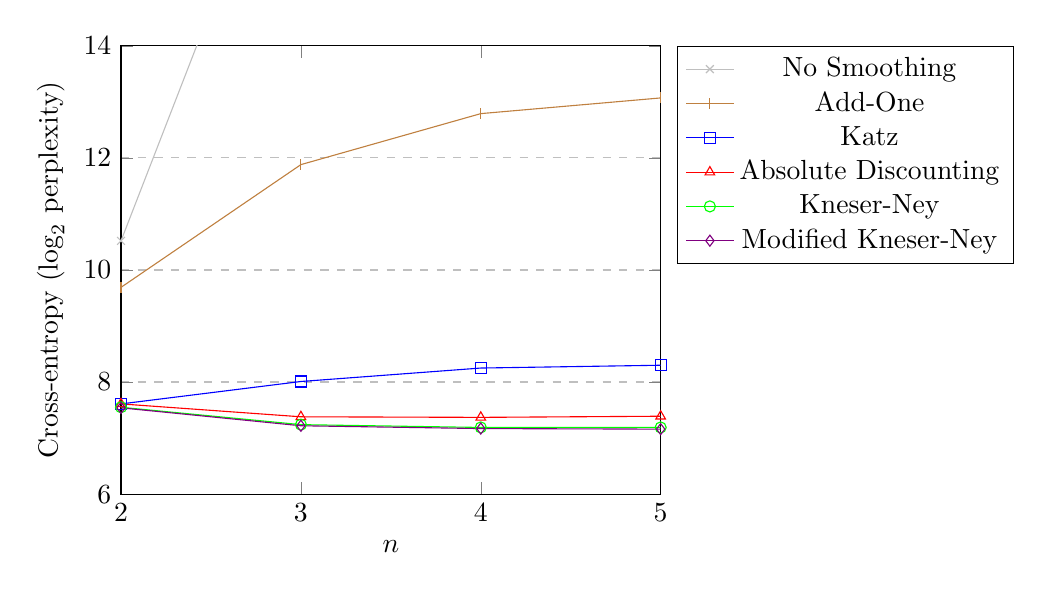
\begin{tikzpicture}[scale=1.0]
\begin{axis}[
	xlabel={$n$},
	ylabel={Cross-entropy ($\log_2$ perplexity)},
	xmin=2, xmax=5,
	ymin=6, ymax=14,
	xtick={2, 3, 4, 5},
	ytick={6, 8, 10, 12, 14},
	legend pos=outer north east,
	ymajorgrids=true,
	grid style=dashed,
]

\addplot[color=lightgray, mark=x]
coordinates {(2, 10.52)(3, 18.79)(4, 24.95)(5, 27.55)};

\addplot[color=brown, mark=|]
coordinates {(2, 9.69)(3, 11.88)(4, 12.79)(5, 13.07)};

\addplot[color=blue, mark=square]
coordinates {(2, 7.61)(3, 8.01)(4, 8.25)(5, 8.30)};

\addplot[color=red, mark=triangle]
coordinates {(2, 7.61)(3, 7.38)(4, 7.37)(5, 7.39)};

\addplot[color=green, mark=o]
coordinates {(2, 7.55)(3, 7.24)(4, 7.19)(5, 7.19)};

\addplot[color=violet, mark=diamond]
coordinates {(2, 7.54)(3, 7.22)(4, 7.17)(5, 7.16)};

\legend{No Smoothing, Add-One, Katz, Absolute Discounting, Kneser-Ney, Modified Kneser-Ney}
 
\end{axis}
\end{tikzpicture}
\caption{Cross-entropy of $n$-gram models trained on the PTB dataset.}
\end{figure}

Recall from equation (4.2) that cross-entropy is just the binary logarithm of perplexity, and that lower perplexity scores indicate better prediction accuracy. With this in mind, it is clear that modified Kneser-Ney smoothing offers the best prediction performance amongst the $n$-gram models. \\

The change in performance with the value of $n$ is interesting. Intuitively, one might expect that increasing $n$ will always yield better results, because this corresponds to increasing the number of words you use to make a prediction. However, for $n$-gram models with no smoothing, add-one smoothing or Katz smoothing, this is not the case. For $n$-gram models with add-one or no smoothing, this is because they do not employ backoff. At higher values of $n$, $n$-grams are much more sparse, so without any backoff higher $n$-gram models can only rely on sparse counts, resulting is lower probabilities being assigned to plausible sequences of words. Katz smoothing does employ backoff, and achieves much better performance, but it still distributes too much probability to rare $n$-grams.

\subsubsection*{A comparison of RNN-based models with $n$-gram models}

As described in the implementation chapter, I also implemented three RNN-based language models which differ in the RNN cell architecture: vanilla RNN, Gated Recurrent Unit and Long Short-Term Memory.

\begin{itemize}
\item
	Plot perplexity (or cross-entropy) and average-keys-saved as a function of the amount of training data used.
\end{itemize}


\begin{figure}[h]
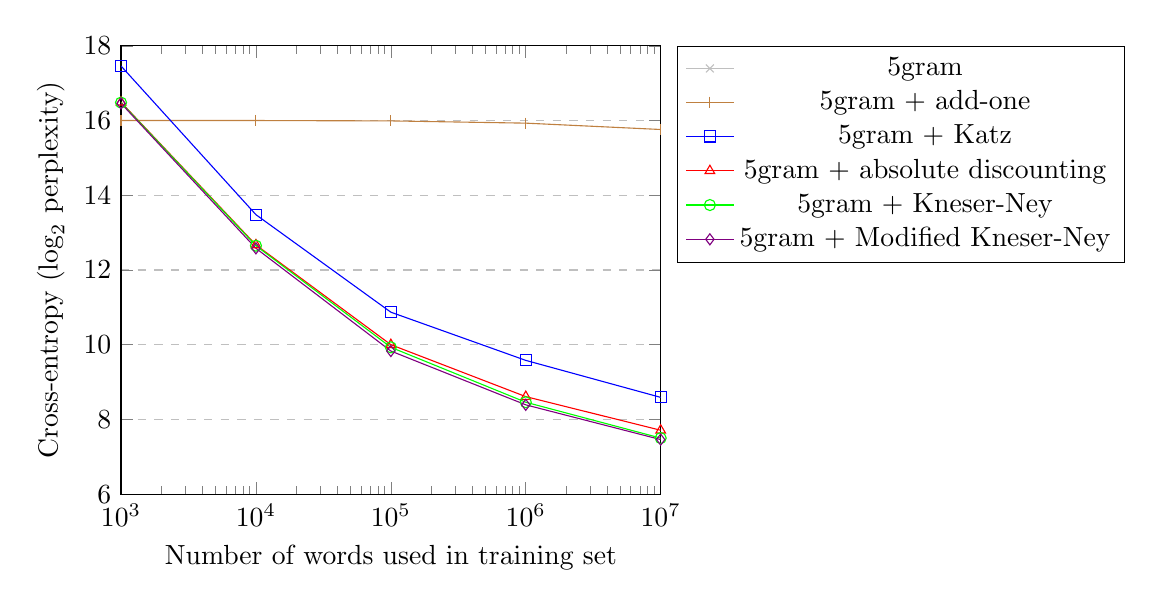
\begin{tikzpicture}[scale=1.0]
\begin{semilogxaxis}[
	xlabel={Number of words used in training set},
	ylabel={Cross-entropy ($\log_2$ perplexity)},
	xmin=1e3, xmax=1e7,
	ymin=6, ymax=18,
	legend pos=outer north east,
	ymajorgrids=true,
	grid style=dashed,
]

% 3gram
%\addplot[color=lightgray, mark=x]
%coordinates {(1e3, 29.33)(1e4, 28.22)(1e5, 25.58)(1e6, 21.29)(1e7, 16.25)};

% 3gram + add-one
%\addplot[color=brown, mark=|]
%coordinates {(1e3, 15.97)(1e4, 15.87)(1e5, 15.59)(1e6, 14.93)(1e7, 13.77)};

% 3gram + Katz
%\addplot[color=blue, mark=square]
%coordinates {(1e3, 17.40)(1e4, 13.48)(1e5, 10.83)(1e6, 9.28)(1e7, 8.14)};

% 3gram + absolute discounting
%\addplot[color=red, mark=triangle]
%coordinates {(1e3, 16.46)(1e4, 12.61)(1e5, 9.92)(1e6, 8.54)(1e7, 7.68)};

% 3gram + Kneser-Ney
%\addplot[color=green, mark=o]
%coordinates {(1e3, 16.45)(1e4, 12.60)(1e5, 9.85)(1e6, 8.41)(1e7, 7.54)};

% 3gram + modified Kneser-Ney
%\addplot[color=violet, mark=diamond]
%coordinates {(1e3, 16.46)(1e4, 12.58)(1e5, 9.84)(1e6, 8.40)(1e7, 7.53)};

% 5gram
\addplot[color=lightgray, mark=x]
coordinates {(1e3, 29.89)(1e4, 29.83)(1e5, 29.58)(1e6, 28.86)(1e7, 27.10)};

% 5gram + add-one
\addplot[color=brown, mark=|]
coordinates {(1e3, 16.00)(1e4, 16.00)(1e5, 15.99)(1e6, 15.93)(1e7, 15.76)};

% 5gram + Katz
\addplot[color=blue, mark=square]
coordinates {(1e3, 17.46)(1e4, 13.48)(1e5, 10.87)(1e6, 9.58)(1e7, 8.59)};

% 5gram + absolute discounting
\addplot[color=red, mark=triangle]
coordinates {(1e3, 16.49)(1e4, 12.67)(1e5, 10.00)(1e6, 8.61)(1e7, 7.71)};

% 5gram + Kneser-Ney
\addplot[color=green, mark=o]
coordinates {(1e3, 16.48)(1e4, 12.65)(1e5, 9.93)(1e6, 8.46)(1e7, 7.50)};

% 5gram + modified Kneser-Ney
\addplot[color=violet, mark=diamond]
coordinates {(1e3, 16.46)(1e4, 12.58)(1e5, 9.83)(1e6, 8.39)(1e7, 7.46)};

\legend{
%	3gram, 3gram + add-one, 3gram + Katz, 3gram + absolute discounting, 3gram + Kneser-Ney, 3gram + Modified Kneser-Ney,
	5gram, 5gram + add-one, 5gram + Katz, 5gram + absolute discounting, 5gram + Kneser-Ney, 5gram + Modified Kneser-Ney,
}
 
\end{semilogxaxis}
\end{tikzpicture}
\caption{Cross-entropy of various language models with respect to the training set size.}
\end{figure}


\begin{figure}[h]
\begin{adjustbox}{center}
\begin{tabular}{| L{5cm} | C{2.5cm} | C{2cm} | C{2cm} | C{2cm} | C{2cm} |}
	\hline
	\tbf{Language Model} & \tbf{Perplexity} & \tbf{Guessing Entropy} & \tbf{Average-Keys-Saved} & \tbf{Memory Usage (MB)} & \tbf{Average Inference Time (ms)} \\ \hline
	3-gram & 4.54 $\times 10^5$$^*$ & 1.97123 & 0.35014 & \tbf{266.91} & 62 \\
	3-gram + add-one & 3764.96 & 1.97123 & 0.53063 & 266.94 & \tbf{41} \\
	3-gram + Katz & 256.95 & 4.45221 & 0.68482 & 266.71 & 88 \\
	3-gram + absolute disc. & 166.03 & 4.10462 & 0.72178 & 266.78 & 63 \\
	3-gram + KN & 150.73 & 4.06848 & 0.72466 & 266.88 & 54 \\
	3-gram + modified KN & 149.54 & 4.08662 & 0.72355 & 266.97 & 54 \\
	5-gram & 1.96 $\times 10^8$$^*$ & 0.23265 & 0.07167 & 737.36 & 130 \\
	5-gram + add-one & 8610.45 & 0.23265 & 0.33886 & 737.30 & 63 \\
	5-gram + Katz & 314.49 & 4.53360 & 0.67154 & 737.43 & 156 \\
	5-gram + absolute disc. & 167.38 & 4.06856 & 0.72333 & 737.43 & 126 \\
	5-gram + KN & 146.35 & 4.01120 & \tbf{0.72598} & 737.37 & 114 \\
	5-gram + modified KN & \tbf{142.68} & 4.03443 & 0.72554 & 737.53 & 116 \\ \hline
	Vanilla RNN 256 & 131.03 & 3.99270 & 0.72776 & 253.67 & 39 \\
	Vanilla RNN 512 & & & & & \\
	GRU 256 & 114.52 & 3.79196 & 0.73993 & 271.39 & 37 \\
	GRU 512 & & & & & \\
	LSTM 256 & 112.47 & 3.84489 & 0.73617 & 287.13 & 38 \\
	LSTM 512 & & & & & \\ \hline
	LSTM 512 interpolated with 5-gram + mod. KN & & & & & \\ \hline
\end{tabular}
\end{adjustbox}
\begin{center}
	{\footnotesize\tit{$^*$These perplexity scores use the approximation mentioned in section 4.1.1 where 0-valued probabilities are replaced with a small constant to avoid division by 0.}}
\end{center}
\caption{A benchmark of various language models on the PTB dataset.}
\end{figure}

Points to discuss:
\begin{itemize}
\item
	Average-keys-saved and guessing entropy taken over first 1000 words, whereas perplexity over whole test set.
\item
	Note $n$-gram models are unpruned (hence large size).
\item
	Katz beaten by absolute-discounting-derived methods on all fronts.
\item
	Modified Kneser-Ney only offers marginal gain in perplexity.
\item
	Reduction in performance of $n$-gram, add-one and Katz with N, due to sparsity of $n$-grams at higher lengths.
\item
	Combination via average.
\item
	Average inference times should be taken with a pinch of salt, because you have to consider CPU scheduling etc.
\end{itemize}

\subsection{On a Mobile Device}

Incorporating an RNN-based language model implementation into a mobile keyboard, as described in section \todo{XXX}, presented a different series of challenges. The strict memory and CPU limitations of App Extensions in iOS forced me to explore the tradeoffs between resource consumption and prediction performance. \\

As shown in figure \todo{XXX}, the vanilla RNN architecture presents the smallest memory overhead, and so this is what I use in the following experiments. I investigated the effect of both vocabulary size and the number of hidden neurons on the memory usage and the average-keys-saved:

\begin{tikzpicture}
\begin{axis}[
	scale only axis,
	xmin=0,xmax=5,
	ymin=0,ymax=1,
	axis y line=left,
	ymajorgrids=true,
	grid style=dashed,
	xlabel=Minimum frequency,
	ylabel=Average-keys-saved]
\end{axis}
\begin{axis}[
	scale only axis,
	xmin=0,xmax=50,
	ymin=0,ymax=1,
	axis x line=top,
	axis y line=none,
	xmajorgrids=true,
	grid style=dashed,
	xlabel=Memory (MB)]
\end{axis}
\end{tikzpicture}


Here, I want to focus on the tradeoff between accuracy and resource consumption. Specifically, I could look at the following: \\
\begin{itemize}
\item
	The effect of increasing the minimum frequency for a word to be considered in the vocabulary. (I.e. the effect of changing the vocabulary size).
\item
	The effect of changing the number of hidden layer neurons.
\item
	The effect of using RNN vs GRU vs LSTM.
\item
	(Perhaps also the effect of pruning on $n$-gram models).
\item
	ALSO: Perhaps compare using float 32 vs float 16 in terms of memory vs accuracy.
\end{itemize}
\subsubsection*{The trade-off between the vocabulary size and resource usage}
\subsubsection*{The trade-off between the number of hidden neurons and resource usage}
\subsubsection*{The trade-off between the number of hidden neurons and resource usage}

Other optimisations (not graphed):
\begin{itemize}
\item
	Remove softmax layer.
\item
	Store weights as float 16 rather than float 32.
\end{itemize}

\subsection{On Error-Prone Text}

I split the CLC dataset up into six files:
\begin{center}
\begin{tabular}{c c}
	\ttt{train.correct.txt} & \ttt{train.incorrect.txt} \\
	\ttt{valid.correct.txt} & \ttt{valid.incorrect.txt} \\
	\ttt{test.correct.txt} & \ttt{test.incorrect.txt}
\end{tabular}
\end{center}
The training, validation and test sets all consisted of one file containing uncorrected text and another file containing the corresponding corrected text. I trained an 2-layer LSTM-based language model with 256 hidden neurons on \ttt{train.correct.txt}, and used \ttt{valid.correct.txt} to guide the learning rate decay. I filtered the test set files such that they only contained pairs of lines that were not identical and that did not contain any insertion or deletion corrections. \\

Before exploring ways to improve the performance on error-prone text, I first established an approximate upper and lower bound. To obtain the upper bound (i.e. the best possible perplexity), I evaluated the LSTM using \ttt{test.correct.txt} for the input words and \ttt{test.correct.txt} for the target words. and 'In order to establish a rough upper and lower bound on the performance of the LSTM on error-prone text, I first evaluated 

Things I aim to evaluate here are: \\

\begin{itemize}
\item
	The hypothetical upper and lower bounds on accuracy (i.e. the LM results on correct input and on incorrect input respectively).
\item
	The effect of using the vocabulary vs different sized dictionaries for determining if a word should be replaced or not.
\item
	The effect of edit distance on performance.
\item
	An intuitive explanation behind the gap remaining between the current performance and the upper bound. Perhaps some suggestions for future work.
\end{itemize}

\begin{figure}[h]
\begin{center}
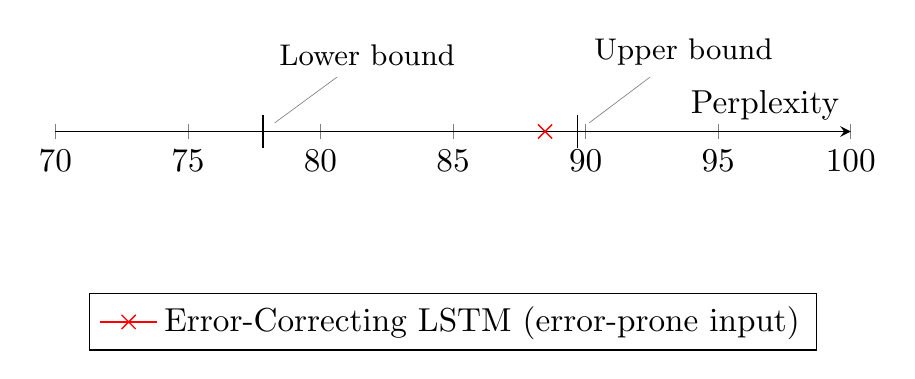
\begin{tikzpicture}[scale=1.2]
\pgfplotsset{every axis legend/.append style={
	at={(0.5, -0.5)},
	anchor=north}}
\begin{axis}[
	axis lines = middle,
	width=10cm,
	height=5cm,
	xlabel={Perplexity},
	axis x line=bottom,
	hide y axis,
	xmin=70, xmax=100,
	ymin=0, ymax=5,
	xtick={70, 75, 80, 85, 90, 95, 100},
]

\addplot[color=black, mark=|, mark size=5.0]
coordinates {(89.70, 0)} node[pin=85:{\small Upper bound}]{};

\addplot[color=red, mark=x, mark size=3.0]
coordinates {(88.47, 0)};

\addplot[color=black, mark=|, mark size=5.0]
coordinates {(77.83, 0)} node[pin=85:{\small Lower bound}]{};

\legend{, Error-Correcting LSTM (error-prone input),}
 
\end{axis}
\end{tikzpicture}
\caption{Perplexity on Cambridge Learner Corpus}
\end{center}
\end{figure}

\chapter{Conclusion}

%%%%%%%%%%%%%%%%%%%%%%%%%%%%%%%%%%%%%%%%%%%%%%%%%%%%%%%%%%%%%%%%%%%%%
% the bibliography
\addcontentsline{toc}{chapter}{Bibliography}
\bibliographystyle{ieeetr}
\bibliography{bibliography}

%%%%%%%%%%%%%%%%%%%%%%%%%%%%%%%%%%%%%%%%%%%%%%%%%%%%%%%%%%%%%%%%%%%%%
% the appendices
\appendix

\chapter{Project Proposal}

\end{document}
